%% \documentclass[final,5p,times]{elsarticle}
\documentclass[final,5p,times,twocolumn]{elsarticle}

\usepackage{graphicx}
\usepackage{amsmath,amsfonts,bm,upgreek}
\usepackage{booktabs,multirow}
\usepackage{subcaption}
\usepackage{xcolor}
\usepackage{float}
\usepackage{enumitem}
\usepackage{makecell}
\usepackage{placeins}
\usepackage{wrapfig}
\usepackage{rotating}
\usepackage[inkscapelatex=false]{svg}

% \documentclass[preprint,12pt]{elsarticle}

%% Use the option review to obtain double line spacing
%% \documentclass[authoryear,preprint,review,12pt]{elsarticle}

%% For including figures, graphicx.sty has been loaded in
%% elsarticle.cls.

%% The amssymb package provides various useful mathematical symbols
\usepackage{amssymb}
%% The amsmath package provides various useful equation environments.
\usepackage{amsmath}
%% The amsthm package provides extended theorem environments
%% \usepackage{amsthm}

%% The lineno packages adds line numbers. Start line numbering with
%% \begin{linenumbers}, end it with \end{linenumbers}. Or switch it on
%% for the whole article with \linenumbers.
%% \usepackage{lineno}

\journal{Powder Technology}

\begin{document}

\begin{frontmatter}

%% Title, authors and addresses

%% use the tnoteref command within \title for footnotes;
%% use the tnotetext command for theassociated footnote;
%% use the fnref command within \author or \affiliation for footnotes;
%% use the fntext command for theassociated footnote;
%% use the corref command within \author for corresponding author footnotes;
%% use the cortext command for theassociated footnote;
%% use the ead command for the email address,
%% and the form \ead[url] for the home page:
%% \title{Title\tnoteref{label1}}
%% \tnotetext[label1]{}
%% \author{Name\corref{cor1}\fnref{label2}}
%% \ead{email address}
%% \ead[url]{home page}
%% \fntext[label2]{}
%% \cortext[cor1]{}
%% \affiliation{organization={},
%%             addressline={},
%%             city={},
%%             postcode={},
%%             state={},
%%             country={}}
%% \fntext[label3]{}

\title{Gas Atomization for Additive Manufacturing: Controlling Particle Size Distribution and Sphericity through Process, Nozzle Design, and Gas Flow Physics}

%% use optional labels to link authors explicitly to addresses:
%% \author[label1,label2]{}
%% \affiliation[label1]{organization={},
%%             addressline={},
%%             city={},
%%             postcode={},
%%             state={},
%%             country={}}
%%
%% \affiliation[label2]{organization={},
%%             addressline={},
%%             city={},
%%             postcode={},
%%             state={},
%%             country={}}

\author{} %% Author name

%% Author affiliation
\affiliation{organization={},%Department and Organization
            addressline={}, 
            city={},
            postcode={}, 
            state={},
            country={}}

\begin{abstract}

Gas atomization is widely used for the production of metallic powders for additive manufacturing, where particle size distribution (PSD) and sphericity are key determinants of process performance. This review examines the relationships between process parameters, nozzle geometry, and resulting powder characteristics, with particular emphasis on the control of PSD and particle shape. After a brief overview of powder production routes, the influence of melt conditions, gas environment, and operating parameters on atomization behavior is discussed. Special attention is given to nozzle design as a governing factor of gas flow structure and fragmentation mechanisms. Fundamental aspects of gas dynamics, including compressible flow and nozzle exit velocity, are revisited to provide a physical basis for understanding these effects. The review highlights key mechanisms linking process conditions to powder morphology, identifies current limitations in predictive approaches, and outlines perspectives for process optimization in additive manufacturing.

\end{abstract}

%%Graphical abstract
\begin{graphicalabstract}
%\includegraphics{grabs}
\end{graphicalabstract}

%%Research highlights
\begin{highlights}
\item Research highlight 1
\item Research highlight 2
\end{highlights}

%% Keywords
\begin{keyword}
Gas atomization \sep Metallic powders \sep Additive manufacturing \sep Particle size distribution \sep Nozzle design \sep Powder morphology \sep Flow dynamics

%% PACS codes here, in the form: \PACS code \sep code
%% MSC codes here, in the form: \MSC code \sep code
%% or \MSC[2008] code \sep code (2000 is the default)

\end{keyword}

\end{frontmatter}

%% Add \usepackage{lineno} before \begin{document} and uncomment 
%% following line to enable line numbers
%% \linenumbers



\section{Introduction}
\label{}

Since its commercialization in the late 20th century, additive manufacturing (AM) has experienced rapid growth, leading to a significant increase in the demand for high-quality metallic powders~\cite{Feng2024PreparationAdditive}. Numerous processes have been developed to produce metallic powders, each offering different levels of productivity, cost, and powder quality, which inherently determine their suitability for specific applications.

Among the key powder characteristics, particle size distribution (PSD) and particle sphericity play a central role, as they directly influence powder flowability, packing density, and process stability. In powder 
bed-based AM processes, such as laser powder bed fusion, variations in powder morphology can lead to poor layer uniformity, defect formation, and variability in the mechanical properties of the final components.
\textcolor{red}{References ``influence powder quality for LPBF''}
Consequently, controlling powder characteristics during production is of critical importance.

Gas atomization has emerged as the predominant method for producing metallic powders for AM applications due to its flexibility, scalability, and its ability to generate relatively spherical particles with controlled size distributions. Over the past decades, extensive research has been conducted on various atomization processes, including vacuum induction melting gas atomization (VIGA)~\cite{Neikov2009HandbookNonFerrous,Kassym2020AtomizationProcesses,Singh2001StudyFree,Goudar2017EffectAtomization,Zou2021PrebreakupMechanism,Ting2002EffectWakeclosure,Wang2024PreciseControl}, electrode induction gas atomization (EIGA), plasma-based processes~\cite{Dion2018PlasmaApparatus,Liu2020BriefIntroduction,Zhao2020CentrifugalGranulation}, water atomization~\cite{Seki1990EffectAtomization}, centrifugal atomization,~\cite{Wu2025ReviewMetal,Zhang2017ParticleSize,Suastiyanti2021DesigningCentrifugal,Zhao2023EffectsProcess,Qiu2012StudyNew} and  processes as ultrasonic atomization~\cite{Balasz2024InvestigationMetal,Ciftcli2025AlloyDevelopment,Priyadarshi2024NewInsights,Wisutmethangoon2011ProductionSAC305} and spray forming \textcolor{red}{references ``spray forming''}.

In the field of gas atomization, a large body of work has focused on characterizing specific experimental setups, operating conditions, and resulting powder properties, while review papers typically synthesize existing knowledge within well-defined technological frameworks. In contrast, this work adopts a more integrative perspective by combining insights from different atomization approaches and by incorporating complementary studies drawn from related research areas. In addition, recent developments in adjacent fields are considered in order to broaden the discussion and highlight transferable physical mechanisms governing powder formation.

In addition, although the thermophysical behavior of gases is well established in fluid mechanics, it is often fragmented across different sources when applied to gas atomization. For this reason, this work introduces a concise and unified presentation of the fundamental gas dynamics relevant to atomization processes, including ideal gas relations, specific heat ratios, speed of sound, and compressible flow through nozzles. This pedagogical approach, supported by explicit graphical representations and derivations, aims to provide a self-contained framework that directly connects gas properties to nozzle exit conditions and momentum transfer. This is particularly relevant for researchers entering the field, as such information is often dispersed across multiple specialized references.

Furthermore, a dedicated synthesis of gas nozzle designs is provided, covering a range of configurations proposed in the literature for improving atomization efficiency and controlling particle formation. Comparative analysis of these geometries highlights the role of flow focusing, gas–liquid interaction, and turbulence generation in determining droplet breakup behavior and resulting powder characteristics.

Building on these elements, this review aims to go beyond a classical process description by integrating a comparative perspective across atomization technologies, a unified physical description of gas flow in atomization, and a critical analysis of nozzle design strategies. The final objective is to identify the most influential parameters governing particle size distribution and sphericity, and to establish a clearer basis for process optimization in gas atomization for additive manufacturing applications.

\section{Powder Production Routes}
\label{s:Powder_Production_Routes}


\subsection{Vaccum Induction Melting Gas Atomization (VIGA)}
\label{s:VIGA}

See Figure~\ref{f:free_fall_confined}

\begin{figure}
    \centering
        \includesvg[width=\columnwidth]{./img/freefall_confined.svg}
        \caption[Free fall and confined gas atomization]{Free fall and confined gas atomization. a) Free fall gas atomization b) Confined gas atomization. $\alpha$ is the apex angle between the liquid metal stream axis and the gas jet axis, $d_{1}$ is the vertical distance between the bottom of the crucible and the gas impact point, and $d_{2}$ is the distance between the gas nozzle output and the impact point. Adapted from~\cite{Goudar2017EffectAtomization}.}
        \label{f:free_fall_confined}
\end{figure}

\subsection{Electrode Induction / Plasma Inert Gas Atomization (EIGA / PIGA)}
\label{s:EIGA_PIGA}

See Figure~\ref{f:eiga_piga}

\begin{figure}
    \centering
        \includesvg[width=\columnwidth]{./img/EIGA_PIGA.svg}
        \caption[EIGA and PIGA processes]{a) EIGA process. Adapted from~\cite{Spitans2020NumericalModeling}. b) PIGA process. Adapted from~\cite{Sun2017ReviewMethods,Chen2018ComparativeStudy}.}
        \label{f:eiga_piga}
\end{figure}

\subsection{Plasma Rotating Electrode Process (PREP)}
\label{s:PREP}

See Figure~\ref{f:prep}

\begin{figure}
    \centering
        \includesvg[width=7cm]{./img/PREP.svg}
        \caption[Plasma Rotating Electrode Process (PREP)]{Plasma Rotating Electrode Process (PREP). Adapted from~\cite{Chen2018ComparativeStudy, Zhao2020CentrifugalGranulation,Wu2025ReviewMetal}.}
        \label{f:prep}
\end{figure}

\subsection{Water Atomization}
\label{s:Water_Atomization}

See Figure~\ref{f:water_nozzle}


\begin{figure}
    \centering
        \includesvg[width=6.5cm]{./img/water_nozzle.svg}
        \caption[Cone and V-jet nozzles for water atomization.]{Cone and V-jet nozzles for water atomization. a) Cone nozzle b) V-jet nozzle. Adapted from~\cite{Seki1990EffectAtomization, Neikov2009HandbookNonFerrous}.}
        \label{f:water_nozzle}
\end{figure}

\subsection{Centrifugal Atomization}
\label{s:Centrifugal_Atomization}

\subsection{Ultrasonic Atomization}
\label{s:Ultrasonic_Atomization}

\subsection{Physical Vapor Deposition (PVD) / Chemical Vapor Deposition (CVD)}
\label{s:PVD_CVD}

\subsection{Combined process for metal powder production}
\label{s:Combined_Process}

\subsection{Cross-Disciplinary Processes}
\label{s:Cross_Disciplinary}

\subsubsection{Mechanical Attrition}
\label{s:Mechanical_Attrition}

\subsubsection{Spray Forming}
\label{s:Spray_Forming}

\subsubsection{Rocket Fuel Atomization}
\label{s:Rocket_Fuel_Atomization}

See Figure~\ref{f:coaxial_swirl}

\begin{figure}
    \centering
        \includesvg[width=6.5cm]{./img/coaxial_swirl.svg}
        \caption{Liquid-liquid coaxial swirl injector designed by Copenhagen Suborbitals. Adapted from~\cite{CopenhagenSuborbitals}.}
        \label{f:coaxial_swirl}
\end{figure}

\subsection{Powder Quality Comparison of Production Routes}
\label{s:Powder_Quality_Comparison}

\begin{itemize}
  \item Heat map of the powder production routes, see Figure~\ref{f:production_routes}
\end{itemize}

\begin{figure}
    \centering
        \includesvg[width=\columnwidth]{./img/codes/production_routes.svg}
        \caption{Comparative Assessment of Powder Production Routes}
        \label{f:production_routes}
\end{figure}

\section{Gas Environment and Flow Fundamentals for Atomization}

\begin{itemize}
  \item Intro context importance to care about controlled atmosphere and inert gas
\end{itemize}

Table~\ref{t:gas_properties} presents a list of inert gases with some properties that can be relevant for the atomization process.

    \begin{table*}
        \centering
       \begin{tabular}{l c c c c c c}
\toprule
            \textbf{Property}     &      \textbf{Helium}     &      \textbf{Neon}          &        \textbf{Argon}    &  \textbf{Krypton} & \textbf{Xenon} & \textbf{Nitrogen}   \\                
\midrule
        \makecell[l]{Molar mass \\ $M$ (g/mol)}       &  4.00$^{a)}$  &   20.18$^{a)}$  &   39.95$^{a)}$ &  83.8$^{a)}$ & 131.3$^{a)}$ & 28.0$^{a)}$ \\
        \makecell[l]{Critical temp. \\ $T_{cr}$ (K)}  & 5.2$^{a)}$  &   44.5$^{a)}$  &   150.7$^{a)}$ & 209.5$^{a)}$ & 289.7$^{a)}$ & 126.2$^{a)}$ \\               
        \makecell[l]{Critical pressure \\ $P_{cr}$ (MPa)} &  0.2275$^{a)}$  &    2.678$^{a)}$  &    4.863$^{a)}$ &  5.51$^{a)}$ & 5.84$^{a)}$ &     3.396$^{a)}$ \\                 
        \makecell[l]{Critical mol. vol. \\ $V_{cr}$ (cm³/mol)}       & 57.48$^{a)}$  &    41.87$^{a)}$  &   74.59$^{a)}$ & 92.25$^{a)}$ & 118.28$^{a)}$ & 89.41$^{a)}$ \\
        \makecell[l]{Critical density    \\ $\rho_{cr}$ (kg/m³)}    & 69.64$^{a)}$  &   481.9$^{a)}$  &    535.6$^{a)}$ & 908.4$^{a)}$ & 1110$^{a)}$ & 313.3$^{a)}$ \\                   
\midrule    
            Specific heat ratio [$\gamma$] &   &   &   &   &   &   \\
            0.1 MPa, 283 K   &  NA & NA  & NA  & NA  &  NA & 1.4$^{d)}$ \\                                  
            0.1 MPa, $<$ 400 K  & 1.67$^{b)}$ & 1.67$^{b)}$ & 1.67$^{b)}$ & 1.67$^{a)}$ & 1.67$^{a)}$ & NA \\
            2 MPa, 400 K     &  1.67$^{c)}$ & 1.67$^{c)}$ & 1.7$^{b)}$  & 1.72$^{b)}$  & 1.79$^{b)}$  & NA \\    
            2 MPa, 1200 K    & 1.67$^{c)}$  & 1.67$^{c)}$  & 1.67$^{c)}$  & 1.7$^{c)}$  & 1.79$^{c)}$  &  NA\\
            7 MPa, 400 K     & 1.66$^{c)}$  &  1.67$^{c)}$ & 1.77$^{b)}$  & 1.88$^{b)}$  & 2.21$^{b)}$  & NA \\
            7 MPa, 1200 K     & 1.66$^{c)}$  & 1.66$^{c)}$  & 1.66$^{c)}$ & 1.67$^{c)}$  &  1.69$^{c)}$   & NA \\
 \midrule                     
            Reactivity      &  1  & 2  & 3  & 4 & 5 & 6 \\
            Price           & 3     &   4    &  2      & 5    & 6   & 1 \\
\bottomrule
\end{tabular}
        \caption[Summary table of gas properties]{Summary table of gas properties. a)~\cite{Tournier2008PropertiesHelium}, b)~\cite{Tournier2008PropertiesNoble}, c) Data visualization reading from~\cite{Tournier2008PropertiesNoble}, d)~\cite{BrinkworthRatiosSpecific}. For the reactivity and price, a 1 to 6 scale is proposed as a general information, ``1'' means lowest price and reactivity, ``6'' means highest price and reactivity. The accurate values depend on other parameters such as the purity of the gas. The nitrogen is chemically stable but can be reactive at high temperature.}
        \label{t:gas_properties}
    \end{table*}

\begin{itemize}
  \item Relation between gaz price and percentage in the atmosphere, see Table~\ref{t:air_composition} in~\ref{a:gas_environment}.
\end{itemize}


\begin{itemize}
  \item 3D Plot "Gas density / pressure / temperature"
\end{itemize}

See Figure~\ref{f:PV_3D}


\begin{figure}
    \centering
        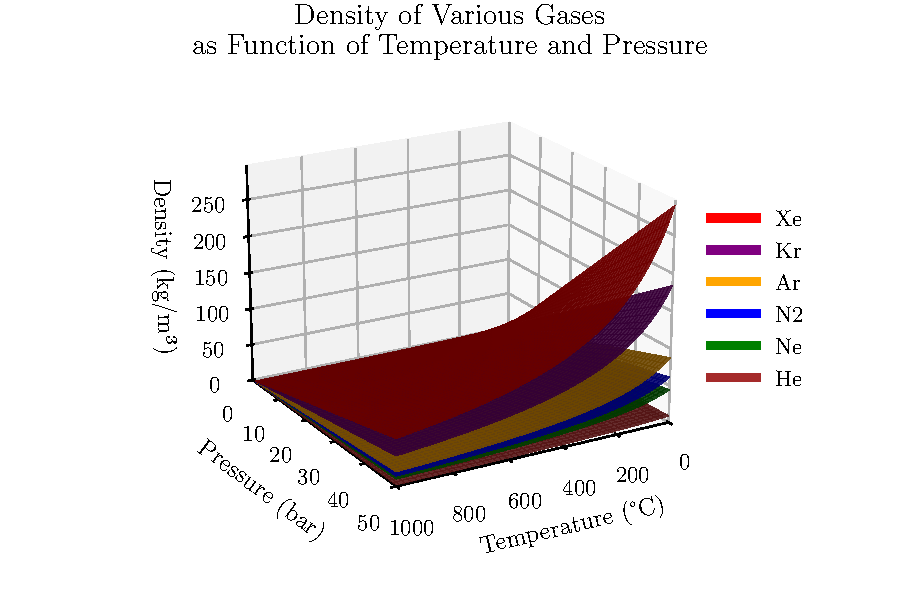
\includegraphics[width=9cm,
        trim= 30 20 30 0, clip]{./img/codes/PV=nRT_3D.pdf}
        \caption{3D plot of the density of the helium, neon, argon, krypton, xenon and nitrogen as a function of temperature and pressure. Molar mass from~\cite{Tournier2008PropertiesHelium}.}
        \label{f:PV_3D}
\end{figure}

\begin{itemize}  
\item 2D plot "speed of sound / temperature"
\end{itemize}

See Figure~\ref{f:speed_of_sound}

\begin{figure}
    \centering
        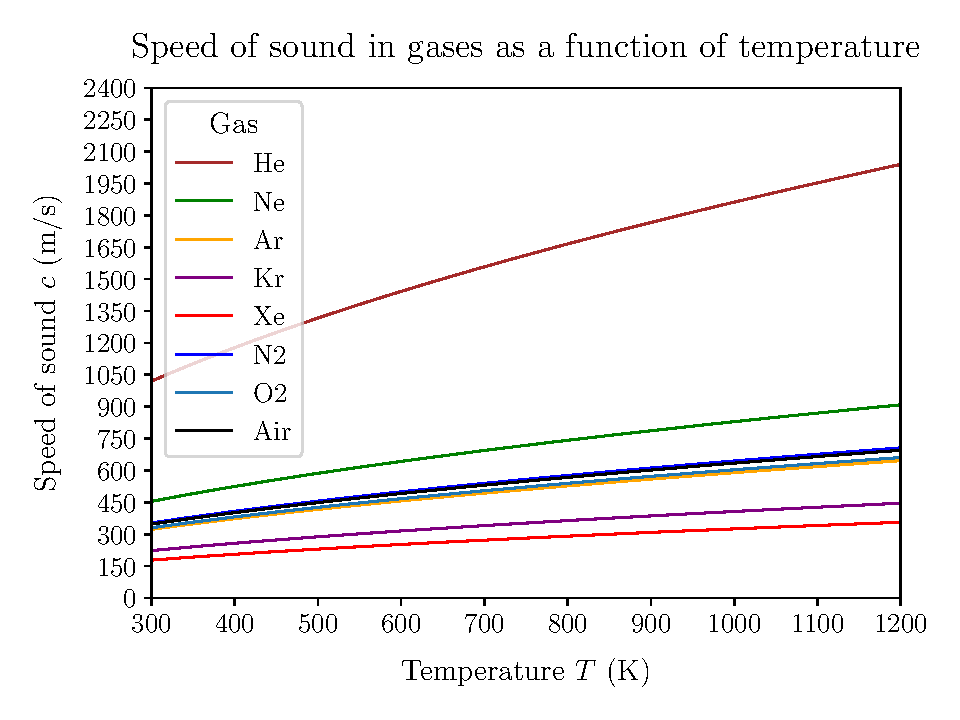
\includegraphics[width=\columnwidth]{./img/codes/speed_of_sound.pdf}
        \caption[Speed of sound in various gases as a function of temperature]. {Speed of sound in various gases as a function of temperature. The speed of sound is calculated using the Formula~\ref{e:speed_of_sound}. The molar mass and specific heat ratio values are taken from Table~\ref{t:gas_properties}, with $\gamma$ at 0.1 MPa and $>$400~K for He, Ne, Ar, Kr and Xe, and $\gamma$ at 0.1 MPa and 283 K for N$_2$. The air properties are calculated taking only nitrogen, oxygen and argon, with the percentage of Table~\ref{t:air_composition}. $M_{oxygen}$ is given by NIST~\cite{Chase1998NISTJANAFThemochemical} and $\gamma_{oxygen}$ is estimated at 1.4 as a diatomic molecule. In this plot, the specific ratio are considered constant as a function of the temperature.}
        \label{f:speed_of_sound}
\end{figure}

\begin{itemize}
  \item Explanation of the results, behavior of monatomic vs diatomic gases (figure and formulas) (appendix?)
\end{itemize}

See Figure~\ref{f:DOF}

\begin{figure}
    \centering
        \includesvg[width=\columnwidth]{./img/DOF.svg}
        \caption[Degrees of freedom of helium and nitrogen molecules]{Degrees of freedom of helium and nitrogen molecules. a) Helium is a monatomic gas, it has 3 degrees of freedom (translation). b) Nitrogen is a diatomic gas, it has 5 degrees of freedom (3 translations and 2 rotations). The rotation around the molecular axis is considered negligible since the moment of inertia is almost zero. The vibration degree of freedom is only activated at high temperatures. Adapted from~\cite{More2020DegreeFreedom}.}
        \label{f:DOF}
\end{figure}

\begin{itemize}
  \item Estimation of speed of gas flow through a nozzle, with formulas and 3D plot "gas name / nozzle pressure / velocity" (details in appendix?)
\end{itemize}

See Figure~\ref{f:velocity_nozzle_out}

\begin{figure}
    \centering
        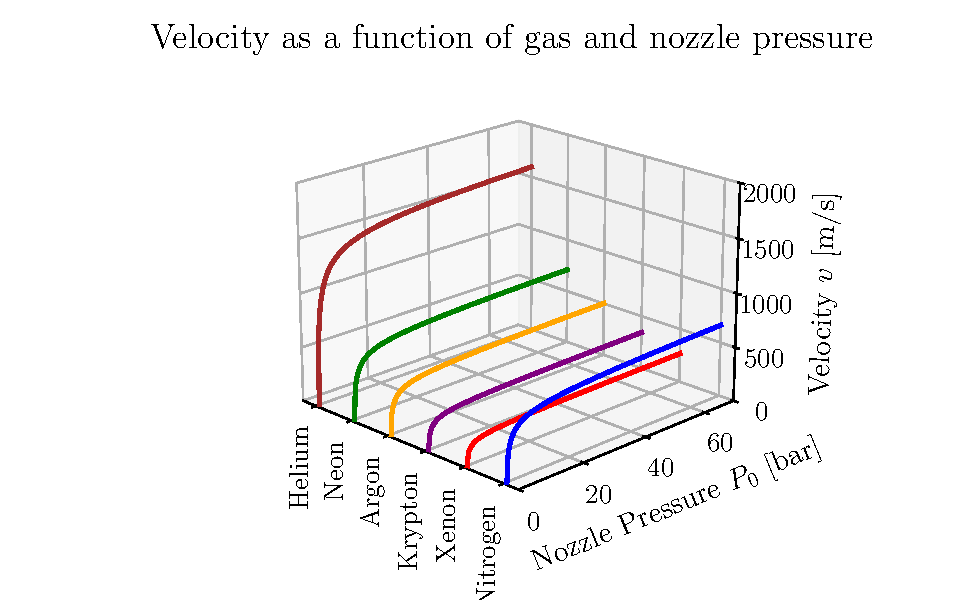
\includegraphics[width=\columnwidth, trim= 30 0 30 0, clip]{./img/codes/velocity_nozzle_out.pdf}
        \caption[Plot of the velocity of different gases at the nozzle outlet as a function of the pressure ratio $P/P_0$ for a given temperature before the nozzle]. {Plot of the velocity of different gases at the nozzle outlet as a function of the pressure ratio $P/P_0$ for a given temperature before the nozzle. Here T$_0$ = 300 K and P = 1 bar. The velocity is calculated using the isentropic flow velocity formula (Equation~\ref{e:isentropic_flow_velocity_gamma}) and the gas properties from Table~\ref{t:gas_properties_velocity}.}
        \label{f:velocity_nozzle_out}
\end{figure}

\begin{itemize}
  \item 3D plot focused on nitrogen "Temperature / nozzle pressure / velocity"
\end{itemize}

See Figure~\ref{f:velocity_nitrogen_3d}

\begin{figure}
    \centering
        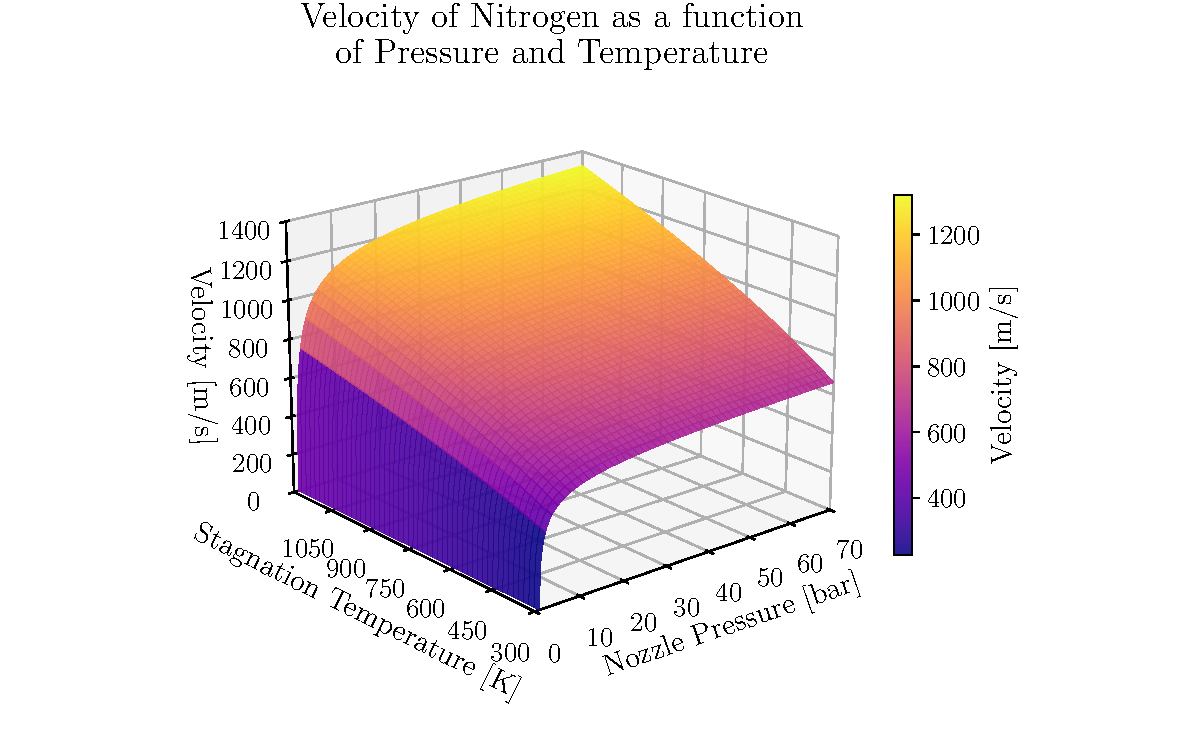
\includegraphics[width=\columnwidth, trim= 60 0 60 0, clip]{./img/codes/velocity_nitrogen_3d.pdf}
        \caption{Velocity of Nitrogen as a function of nozzle pressure and nozzle temperature.}
        \label{f:velocity_nitrogen_3d}
\end{figure}

\begin{itemize}
  \item Example with DTU atomizer conditions
\end{itemize}

\section{Nozzle Geometry and Flow Dynamics}

\begin{itemize}
  \item Explanation of the concept of Gas to metal ratio
  \item Review example of discrete jet vs annular jets
\end{itemize}

See Figure~\ref{f:water_double_stage_nozzle}

\begin{figure}
    \centering
        \includesvg[width=\columnwidth]{./img/water_double_stage_nozzle.svg}
        \caption[Water double stage nozzle]{a) Water double stage nozzle. b) Upper stage nozzle with axial jets. c) Lower stage nozzle with tangential jets. Adapted from~\cite{Neikov2009HandbookNonFerrous}}
        \label{f:water_double_stage_nozzle}
\end{figure}


\begin{itemize}
  \item Review example of Prefilm nozzle and Nanoval nozzle
  \item Description of the concept of Closed-Wake pressure with review example (which has a significant influence on the particle size)
\end{itemize}

See Figure~\ref{prefilm_and_nanoval}

\begin{figure}
    \centering
        \includesvg[width=\columnwidth]{./img/prefilm_and_nanoval.svg}
        \caption[Prefilm and Nanoval nozzle]{a) Prefilm nozzle. b) Nanoval nozzle. Ma is the Mach number. Adapted from~\cite{Neikov2009HandbookNonFerrous,Cacace2024InvestigationEffect}.}
        \label{prefilm_and_nanoval}
\end{figure}


\section{Conclusion}

List of the factor that has to be taken into account to improve the size of particles,PSD, and sphericity.\\

Minor effect:
\begin{itemize}
  \item Gas type
  \item Gas temperature
\end{itemize}

Major effect:
\begin{itemize}
  \item Gas pressure and GMR
  \item Nozzle design
\end{itemize}

Some perspectives for future research on the nozzle design optimizationaccording to litterature:
\begin{itemize}
  \item Reduce outer diam of the melt nozzle
  \item Keep small apex angle
  \item Several stage of atomization
  \item Use of swirl flow
  \item Use of prefilming
  \item Use of annular jets
  \item Use of Laval nozzle
  \item Regime Closed-Wake
\end{itemize}
















% \paragraph{Paragraph Heading}
% \label{}

% \subparagraph{Subparagraph Heading}
% \label{}










\appendix
\section{Gas environnement applied to atomization}
\label{a:gas_environment}

\vspace{0mm}
\begin{table}[H]
    \centering
    \begin{tabular}{l c c}
        \toprule
        \textbf{Component} & \textbf{\% by volume} & \textbf{\% by mass} \\
        \midrule
        Nitrogen, N$_2$ & 78.08 & 75.53 \\
        Oxygen, O$_2$ & 20.95 & 23.14 \\
        Argon, Ar & 0.93 & 1.28 \\
        Carbon dioxide, CO$_2$ & 0.031 & 0.047 \\
        Hydrogen, H$_2$ & $5.0 \times 10^{-3}$ & $2.0 \times 10^{-4}$ \\
        Neon, Ne & $1.8 \times 10^{-3}$ & $1.3 \times 10^{-3}$ \\
        Helium, He & $5.2 \times 10^{-4}$ & $7.2 \times 10^{-5}$ \\
        Methane, CH$_4$ & $2.0 \times 10^{-4}$ & $1.1 \times 10^{-4}$ \\
        Krypton, Kr & $1.1 \times 10^{-4}$ & $3.2 \times 10^{-4}$ \\
        Nitric oxide, NO & $5.0 \times 10^{-5}$ & $1.7 \times 10^{-6}$ \\
        Xenon, Xe & $8.7 \times 10^{-6}$ & $1.2 \times 10^{-5}$ \\
        Ozone, O$_3$ (summer) & $7.0 \times 10^{-6}$ & $1.2 \times 10^{-5}$ \\
        Ozone, O$_3$ (winter) & $2.0 \times 10^{-6}$ & $3.3 \times 10^{-6}$ \\
        \bottomrule
    \end{tabular}
    \caption{The composition of dry air at sea level~\cite{Atkins2022AtkinsPhysical}}
    \label{t:air_composition}
\end{table}
\FloatBarrier
\vspace{0mm}




\bibliographystyle{elsarticle-num} 
\bibliography{PhD}


% \usepackage[
%   backend=biber,
%   style=numeric,
%   sorting=none,
%   doi=true,       
%   url=true        
% ]{biblatex}
% \addbibresource{PhD.bib}
% \DeclareFieldFormat{urldate}{}



\end{document}

\endinput

